\section{[Bonus] The Best Joke on Earth}

To celebrate April Fools (as of the time I write this), let me explain to you one of the biggest jokes on this planet -- the amount of security our school puts on student accounts. While bypassing the school's restriction on certain sites is even more hilarious than this, I feel that this issue is much more dangerous. I hope that by reading this, you'll be able to protect yourself from future attacks and whoever else you may know.

As you may know, student credentials follow this standarized pattern upon a student's enrollment:

\begin{centering}
\texttt{
Username: \{first name\}\{last initial\}\{last 4 digits of ID\} \newline
Password: \{first initial\}\{last initial\}\{birth: MM/DD/YYYY\}
}
\end{centering}

This is unacceptable. If you knew someone's username and birthday, you'll be able to crack this account in 1-2 tries. Even with just the username, only 365 * 6 = 2190 tries are needed at max to guess its password; much less if you guess their birthyear from their classes or know their month of birth. Worst of all, this formula is used for every single student account in the district, so everyone is at risk.

However, it is important to note that the google login page will only let you try only about 6 times before preventing your IP from logging into the account until an email confirms those actions. That means your most likely safe if you don't tell anyone your birthday or username, right? Wrong.

\subsection*{Getting the Username}


\begin{figure}[h]
    \centering
    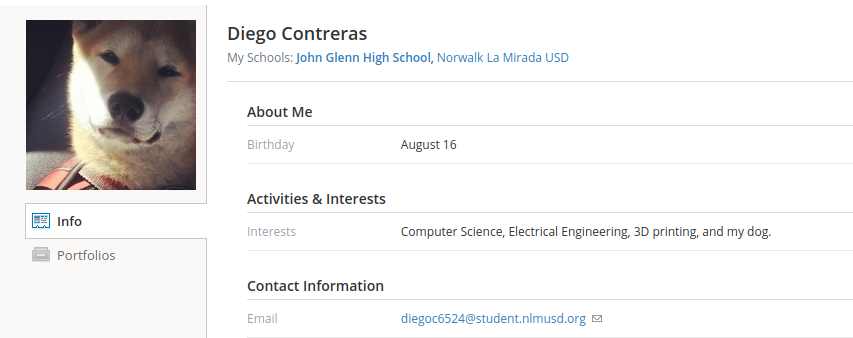
\includegraphics[width=\textwidth,height=3cm,keepaspectratio=true]{School/ProfileEmail}
    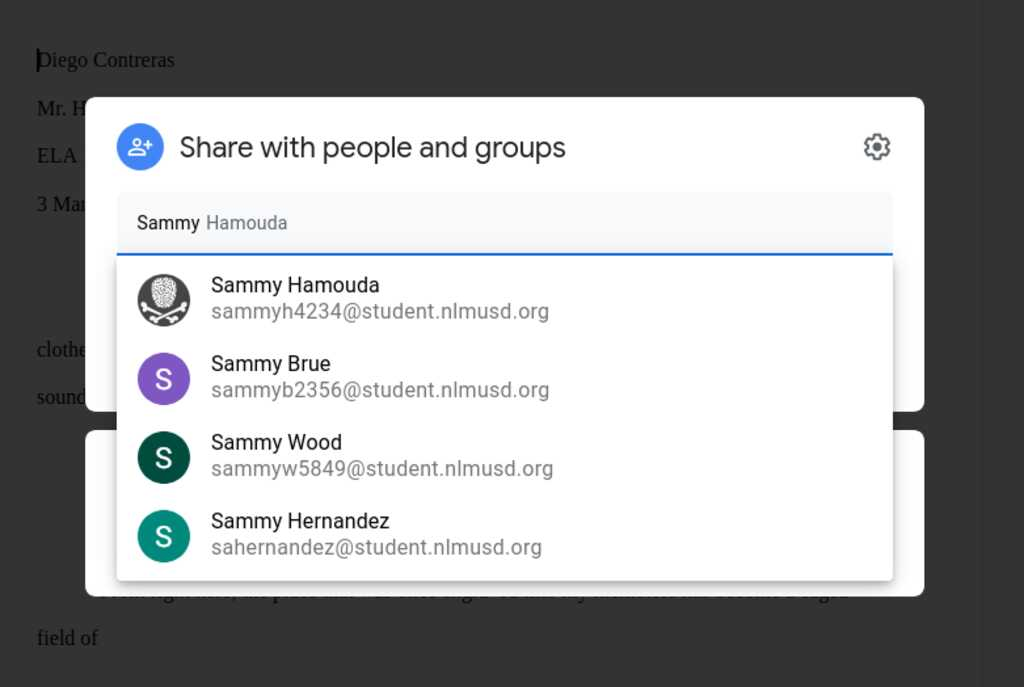
\includegraphics[width=\textwidth,height=3cm,keepaspectratio=true]{School/GoogleEmail}
    \caption{
        (Left) My email AND birthday being shown in my profile. (Right) The result of searching Sammy Hamouda; A good friend of mine who HAS changed his password.
    }
\end{figure}

The username of every single student account is the same that is used in the student's email, period; There's no escape. The fastest way to get a person's email is by simply visiting their profile page on Schoology. Even if the schoology account was set to private, you can SEARCH their email by sharing a google doc or slides with them.

\subsection*{Getting the Password}

\begin{figure}[h]
    \centering
    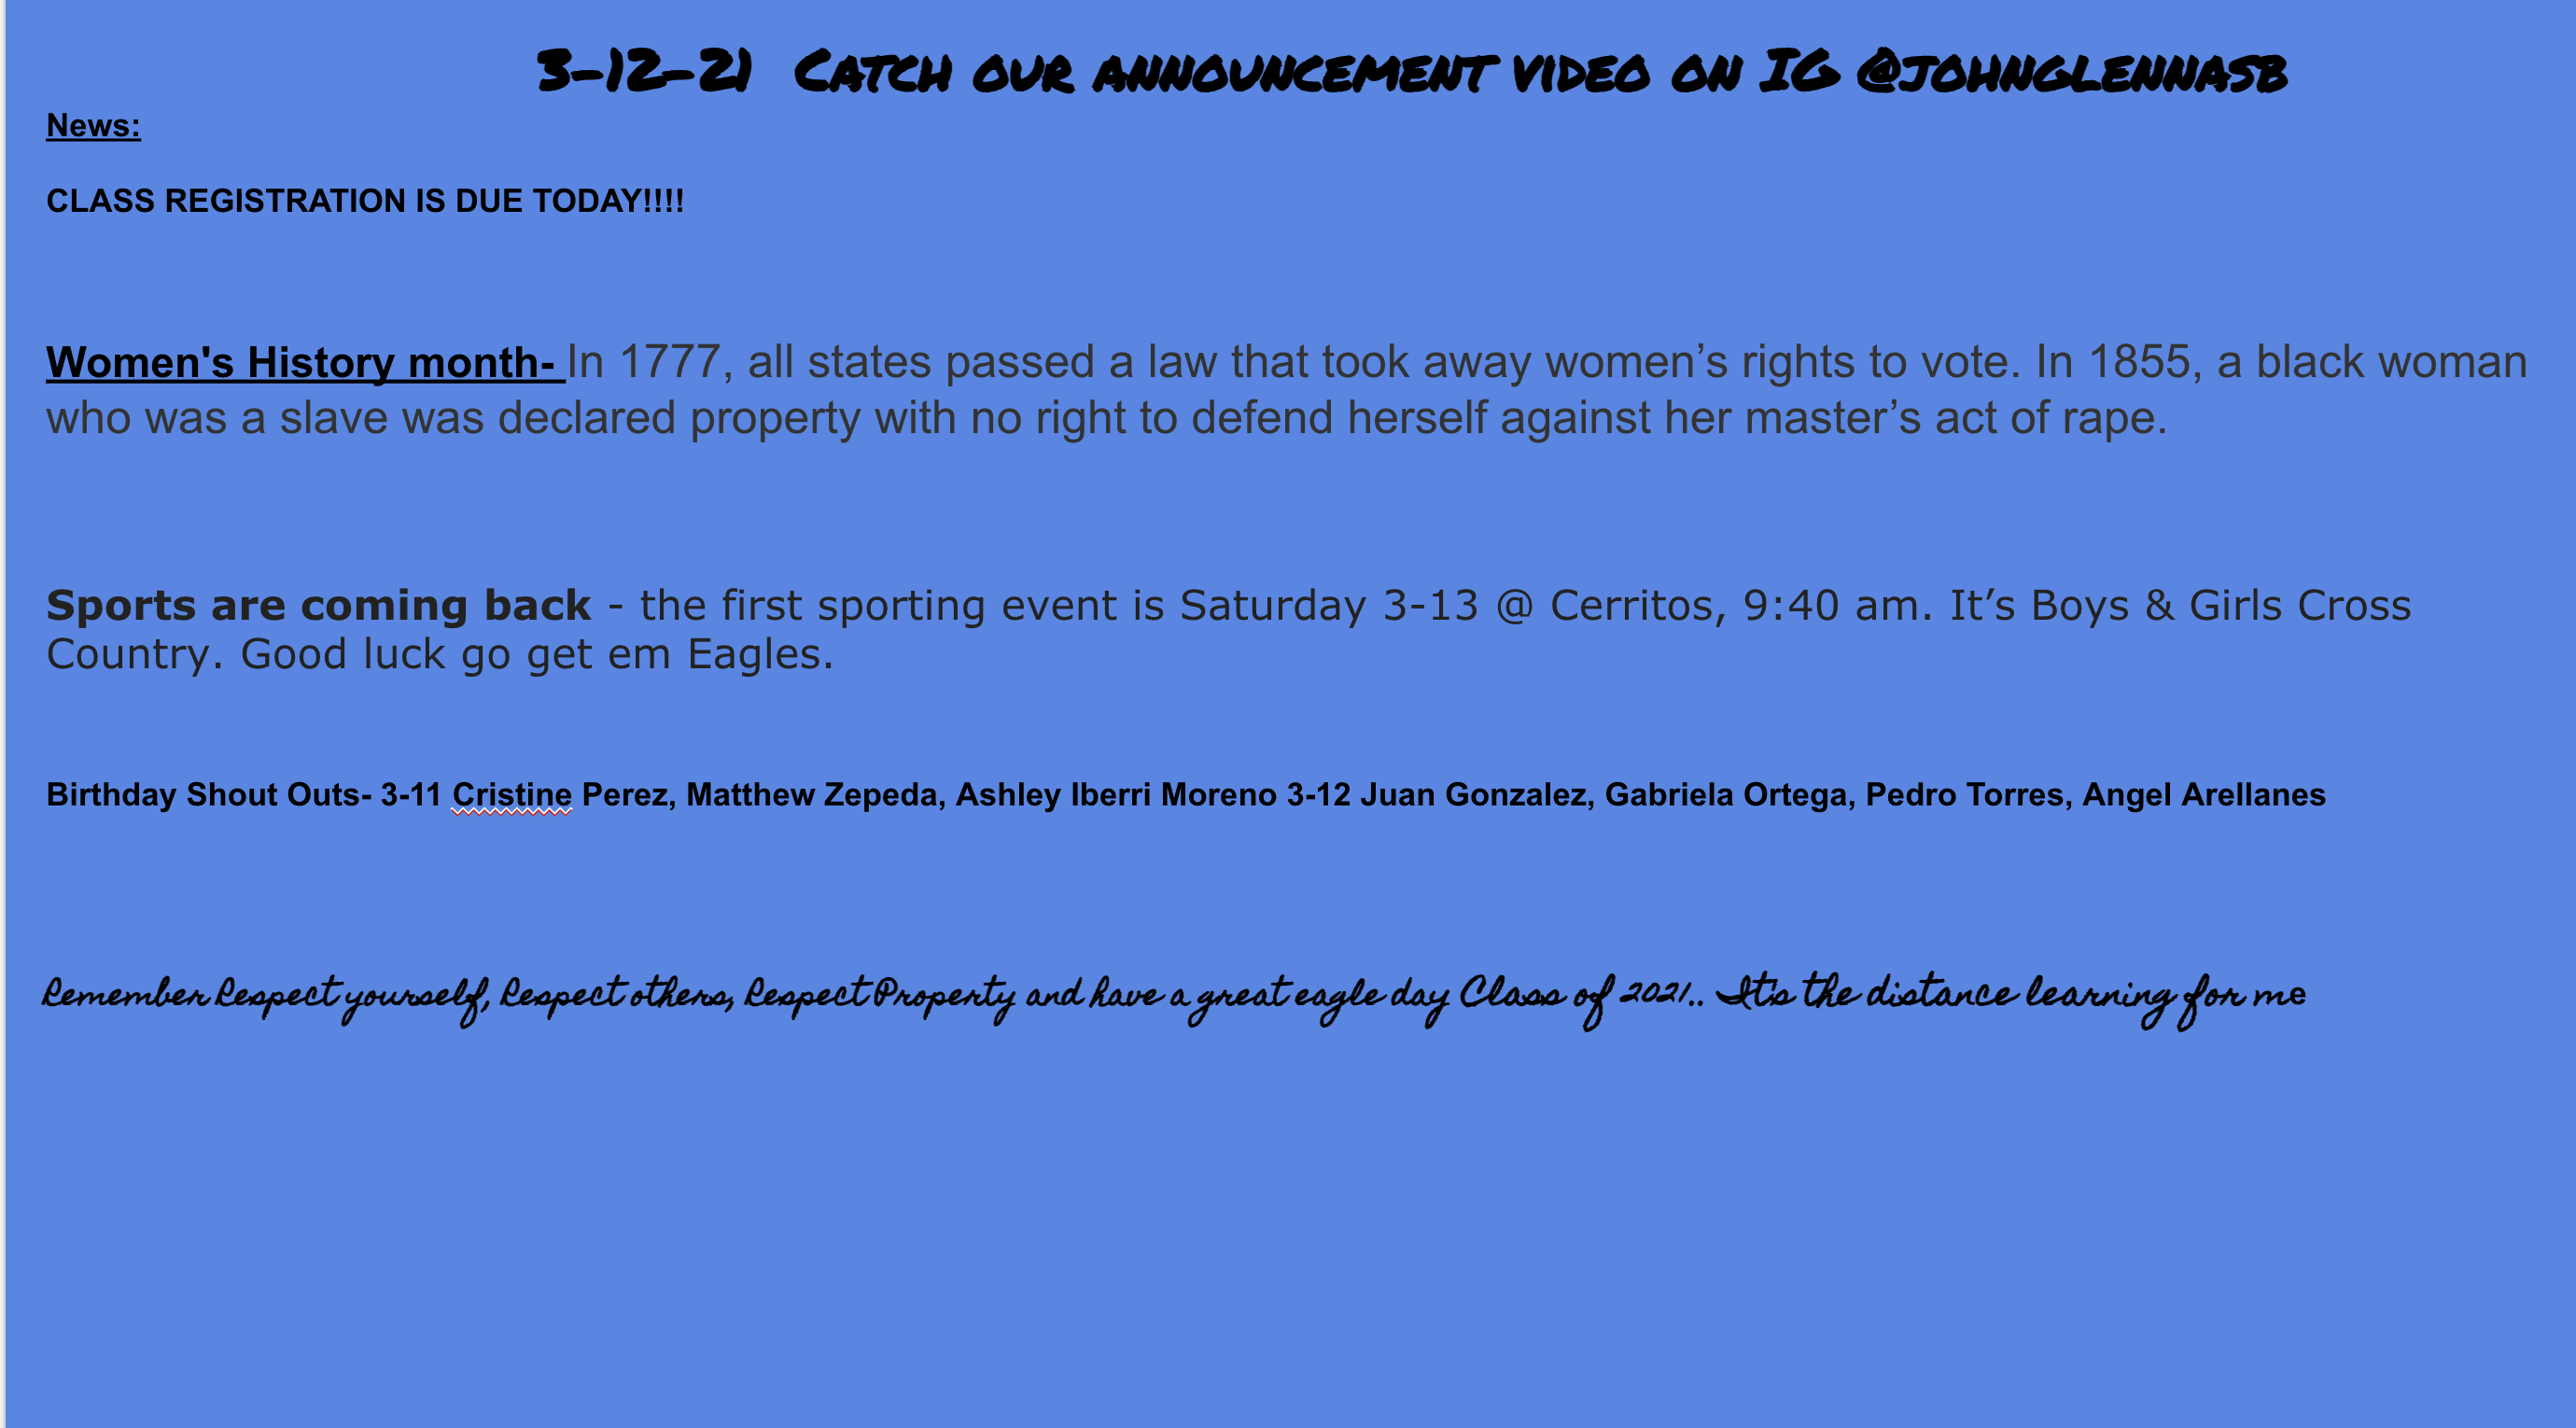
\includegraphics[width=\textwidth,height=6cm,keepaspectratio=true]{School/SchoolAnnouncement}
    \caption{
        Image of just one school announcement exposing 7 birthdays.
    }
\end{figure}


This one's the hardest to get. Really, all you need is to know someone's birth month and day and iterate through all possible years. I estimate that only about 10\% of birthdays are visible on student's schoology accounts in high school and middle school. However, through social media, I bet you can crank that number up to 20\% if their account is public, or around 30\% if you're able to follow them or other means, such as through word of mouth.

I'd say the killer however are school annoucements. Here at JGHS, student birthdays are announced daily. With about 1000 accounts here at the school and about 9 months in a school year, I'd say you'd be able to breach into about 750 accounts if you put in the effort; We're talking about 75\% of accounts being hacked here. Crazy, right?

Even without this in-depth knowledge, more than 700 student accounts in the entire district let you view your birthdays as of December 2020; Trust me, I counted with a very elaborate script.

\subsection*{Brute-forcing}

While google only allows you 6 shots at guessing a password, Powerschool, which uses the same credentials, gives you a seemingly infinite amount of shots (at least 50) in 30 seconds intervals, as tested with my own account. So, if you are really insisted on breaking in on an account, you could, in theory, make a script that guesses all 365 * 6 = 2190 password in less than a day. If you have a chance to look at that person's courses or their overall physique to figure out their year of birth, you could bring that down to just 365 tries that can be cracked in just over 3 hours. This means 100\% of all known student powerschool accounts in the district have the potential to be breached, with 80\% or so of schoology accounts having the same credentials as them.

\textbf{Conclusion: Change your google password. Seriously. Someone can breach into your account at any moment using this method (even applies to those with middle names in a slightly different manner) and use it for hardcore plagirism, identity fraud, and harassment. This is not a joke. If it were, I wouldn't have written this document. I've had several friends complain to me about this.}

\subsection*{Protecting Yourself}

\begin{figure}[h]
    \centering
    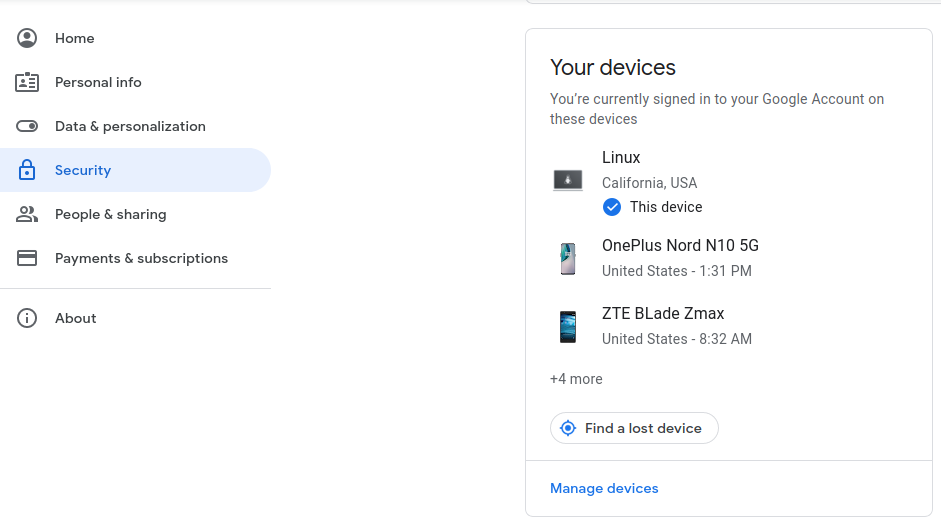
\includegraphics[width=\textwidth,height=4cm,keepaspectratio=true]{School/YourDevicesList}
    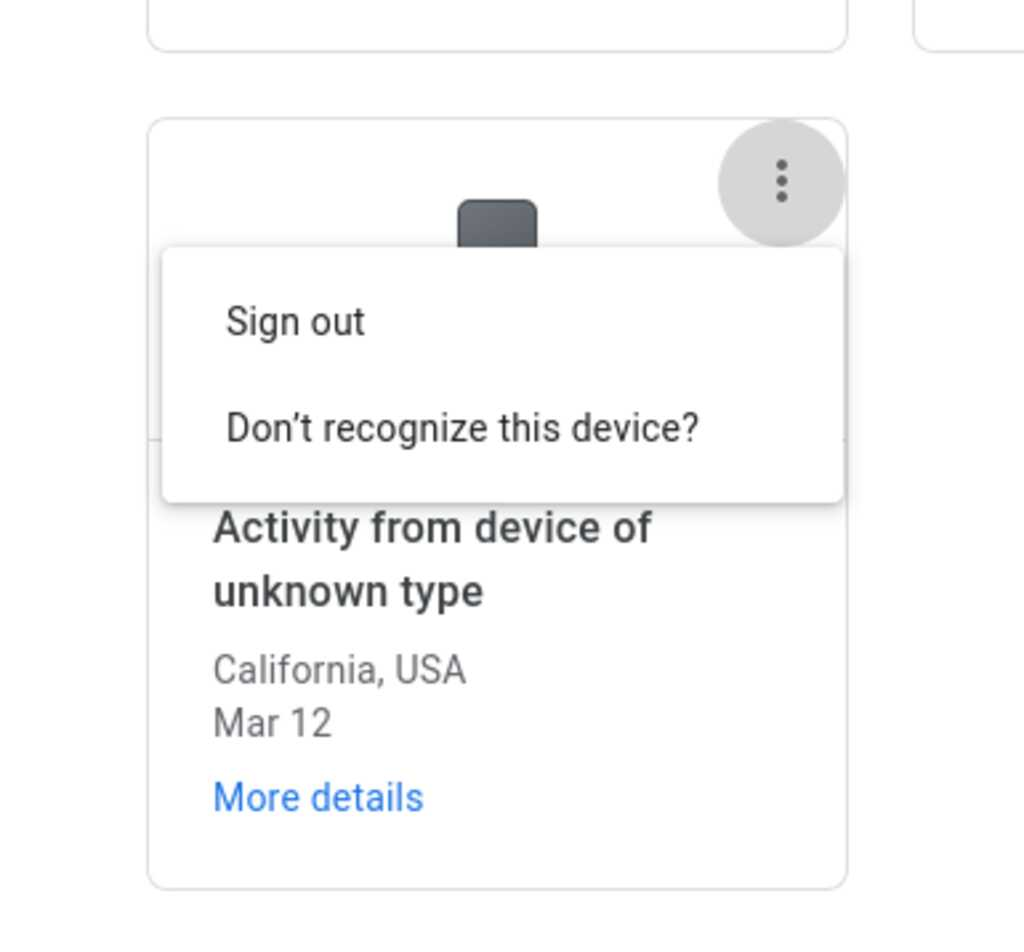
\includegraphics[width=\textwidth,height=4cm,keepaspectratio=true]{School/RemoveDevice}
    \caption{
        (Left) Security $>$ Your Devices (Right) Signing out a device you don't recognize.
    }
\end{figure}

The BEST thing you can do right now is change your google password at this very moment BEFORE hackers do it for you. Even adding a simple underscore in your existing password will prevent 99\% of your slightly more tech literate buddies from hacking into your account. It's that simple; The school couldn't care less.

To get rid of any existing pests, go to Security $>$ Your devices, click on the the three dots of devices you don't recognize, and press Sign Out. This is your first line of defense, and literally signs other people out of your account.

Even with this protection, powerschool accounts are forever breached unless further action is taken. As you may know, changing passwords on your powerschool account is much harder than that of your google account considering grades are vital for you and your parent's information. Due to this, the most amount of damage a person could do if you properly protected yourself is look at your grades and mess with your class enrollment, which is irrelevant to them.
